\documentclass[aspectratio=169]{beamer}
\usetheme{Madrid}
\usecolortheme{default}

% Packages
\usepackage{graphicx}
\usepackage{booktabs}
\usepackage{tikz}
\usepackage{multicol}
\usepackage{amsmath}

% Title information
\title[AI-Generated Image Detection]{AI-Generated Image Detection}
\subtitle{A Comparative Study of CNN Architectures}
\author{Marston Ward \and Victor Salcedo \and Jasper Dolar}
\institute[USD]{
    University of San Diego\\
    Applied Artificial Intelligence: Computer Vision
}
\date{December 8, 2025}

% Custom colors
\definecolor{usdblue}{RGB}{0,102,204}
\definecolor{usdgold}{RGB}{255,197,0}
\setbeamercolor{structure}{fg=usdblue}

\begin{document}

% Title slide
\begin{frame}
    \titlepage
\end{frame}

% Slide 1: Problem & Motivation
\begin{frame}{Problem \& Motivation}
    \begin{columns}[T]
        \begin{column}{0.5\textwidth}
            \textbf{The Deepfake Challenge}
            \begin{itemize}
                \item Synthetic media misrepresented as authentic
                \item Growing threat to digital integrity
                \item Generated using GANs
                \item Enables fraud and misinformation
            \end{itemize}
            
            \vspace{0.5cm}
            \textbf{Why CNNs?}
            \begin{itemize}
                \item Excel at visual pattern recognition
                \item Detect subtle AI artifacts
                \item Transfer learning leverages pretrained features
            \end{itemize}
        \end{column}
        
        \begin{column}{0.5\textwidth}
            \begin{block}{Our Approach}
                \textbf{Comparative Study of 3 Architectures:}
                \begin{enumerate}
                    \item \textcolor{blue}{Custom CNN} - Baseline
                    \item \textcolor{red}{ResNet50} - Transfer learning
                    \item \textcolor{green!60!black}{EfficientNet-B2} - Advanced
                \end{enumerate}
            \end{block}
            
            \vspace{0.3cm}
            \begin{block}{Dataset}
                \begin{itemize}
                    \item 152,710 images (Hugging Face)
                    \item Real vs AI-Generated
                    \item 80/10/10 train/val/test split
                \end{itemize}
            \end{block}
        \end{column}
    \end{columns}
\end{frame}

% Slide 2: Dataset & Methodology
\begin{frame}{Dataset \& Methodology}
    \begin{columns}[T]
        \begin{column}{0.55\textwidth}
            \textbf{Dataset Characteristics}
            \begin{itemize}
                \item \textbf{Source:} Hugging Face
                \item \textbf{Total:} 152,710 images
                \item \textbf{Classes:} Real (0) vs AI-Generated (1)
                \item \textbf{Split:} 122,168 train / 15,271 val / 15,271 test
                \item \textbf{Balance:} Equal class distribution
                \item \textbf{Diversity:} Portraits, animals, objects, scenes
            \end{itemize}
            
            \vspace{0.3cm}
            \textbf{Preprocessing}
            \begin{itemize}
                \item Resize to $224 \times 224$ pixels (RGB)
                \item ImageNet normalization
                \item Data augmentation:
                    \begin{itemize}
                        \scriptsize
                        \item Random horizontal flips
                        \item Random rotation ($\pm 10^\circ$)
                        \item Color jittering
                    \end{itemize}
            \end{itemize}
        \end{column}
        
        \begin{column}{0.45\textwidth}
            \textbf{Training Configuration}
            \begin{table}[h]
                \scriptsize
                \begin{tabular}{ll}
                    \toprule
                    \textbf{Parameter} & \textbf{Value} \\
                    \midrule
                    Hardware & A100 GPU \\
                    Precision & AMP (Mixed) \\
                    Batch Size & 32 \\
                    Workers & 2 \\
                    Test Set & 15,271 images \\
                    \bottomrule
                \end{tabular}
            \end{table}
            
            \vspace{0.3cm}
            \textbf{Key Decisions}
            \begin{itemize}
                \item Balanced dataset reduces bias
                \item ImageNet normalization for transfer learning
                \item Conservative augmentation preserves features
                \item Large test set for robust evaluation
            \end{itemize}
        \end{column}
    \end{columns}
\end{frame}

% Slide 3: Model Architectures
\begin{frame}{Model Architectures}
    \begin{columns}[T]
        \begin{column}{0.33\textwidth}
            \begin{block}{Custom CNN}
                \textcolor{blue}{\textbf{Baseline Architecture}}
                
                \textbf{Design:}
                \begin{itemize}
                    \scriptsize
                    \item 3 Conv blocks
                    \item 32 $\rightarrow$ 64 $\rightarrow$ 128 filters
                    \item BatchNorm + ReLU
                    \item MaxPooling
                    \item FC + Dropout (0.5)
                \end{itemize}
                
                \textbf{Training:}
                \begin{itemize}
                    \scriptsize
                    \item 10 epochs
                    \item Adam (lr=0.001)
                    \item BCEWithLogitsLoss
                    \item 2-3 min/epoch
                \end{itemize}
                
                \textbf{Parameters:}
                \begin{itemize}
                    \scriptsize
                    \item \textbf{2.1M} trainable
                \end{itemize}
            \end{block}
        \end{column}
        
        \begin{column}{0.33\textwidth}
            \begin{block}{ResNet50}
                \textcolor{red}{\textbf{Transfer Learning}}
                
                \textbf{Design:}
                \begin{itemize}
                    \scriptsize
                    \item Pretrained ImageNet
                    \item Frozen backbone
                    \item Custom 2-class head
                    \item Deep residual blocks
                \end{itemize}
                
                \textbf{Training:}
                \begin{itemize}
                    \scriptsize
                    \item 5 epochs
                    \item Adam (lr=$1 \times 10^{-4}$)
                    \item Weight decay=$1 \times 10^{-4}$
                    \item CrossEntropyLoss
                    \item 3-5 min/epoch
                \end{itemize}
                
                \textbf{Parameters:}
                \begin{itemize}
                    \scriptsize
                    \item \textbf{2K} trainable
                    \item 25.6M frozen
                \end{itemize}
            \end{block}
        \end{column}
        
        \begin{column}{0.33\textwidth}
            \begin{block}{EfficientNet-B2}
                \textcolor{green!60!black}{\textbf{Compound Scaling}}
                
                \textbf{Design:}
                \begin{itemize}
                    \scriptsize
                    \item Compound scaling
                    \item Depth + Width + Resolution
                    \item Pretrained frozen backbone
                    \item Efficient architecture
                \end{itemize}
                
                \textbf{Training:}
                \begin{itemize}
                    \scriptsize
                    \item 5 epochs
                    \item Adam (lr=$1 \times 10^{-4}$)
                    \item Weight decay=$1 \times 10^{-4}$
                    \item CrossEntropyLoss
                    \item 4-6 min/epoch
                \end{itemize}
                
                \textbf{Parameters:}
                \begin{itemize}
                    \scriptsize
                    \item \textbf{7.8M} trainable
                    \item 9.1M total
                \end{itemize}
            \end{block}
        \end{column}
    \end{columns}
\end{frame}

% Slide 4: Results & Performance
\begin{frame}{Results \& Performance}
    \begin{columns}[T]
        \begin{column}{0.5\textwidth}
            \textbf{Model Comparison}
            \begin{table}[h]
                \small
                \begin{tabular}{lccc}
                    \toprule
                    \textbf{Model} & \textbf{Accuracy} & \textbf{Parameters} & \textbf{Epochs} \\
                    \midrule
                    \textcolor{blue}{Custom CNN} & \textbf{90.28\%} & 2.1M & 10 \\
                    \textcolor{red}{ResNet50} & 80.32\% & 2K & 5 \\
                    \textcolor{green!60!black}{EfficientNet-B2} & 74.12\% & 7.8M & 5 \\
                    \bottomrule
                \end{tabular}
            \end{table}
            
            \vspace{0.3cm}
            \textbf{Custom CNN Classification Report}
            \begin{table}[h]
                \tiny
                \begin{tabular}{lcccc}
                    \toprule
                    \textbf{Class} & \textbf{Precision} & \textbf{Recall} & \textbf{F1-Score} & \textbf{Support} \\
                    \midrule
                    Real & 0.91 & 0.90 & 0.91 & 8,061 \\
                    AI-Generated & 0.89 & 0.90 & 0.90 & 7,210 \\
                    \midrule
                    \textbf{Accuracy} & & & \textbf{0.90} & \textbf{15,271} \\
                    \bottomrule
                \end{tabular}
            \end{table}
            
            \vspace{0.2cm}
            \begin{itemize}
                \scriptsize
                \item \textbf{Winner:} Custom CNN at 90.28\%
                \item \textbf{Surprise:} Baseline outperforms transfer learning
                \item \textbf{Balance:} Good precision/recall for both classes
            \end{itemize}
        \end{column}
        
        \begin{column}{0.5\textwidth}
            \begin{center}
                \textbf{Test Accuracy Comparison}
                \vspace{0.2cm}
                
                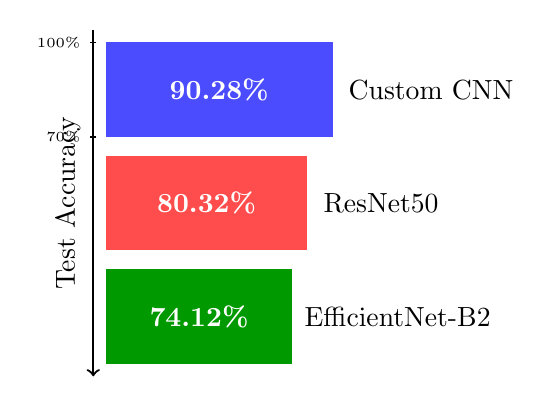
\begin{tikzpicture}[scale=0.8]
                    % Custom CNN bar
                    \fill[blue!70] (0,0) rectangle (3.6,1.5);
                    \node at (1.8,0.75) {\textcolor{white}{\textbf{90.28\%}}};
                    \node[anchor=west] at (3.7,0.75) {Custom CNN};
                    
                    % ResNet50 bar
                    \fill[red!70] (0,-1.8) rectangle (3.2,-.3);
                    \node at (1.6,-1.05) {\textcolor{white}{\textbf{80.32\%}}};
                    \node[anchor=west] at (3.3,-1.05) {ResNet50};
                    
                    % EfficientNet-B2 bar
                    \fill[green!60!black] (0,-3.6) rectangle (2.96,-2.1);
                    \node at (1.48,-2.85) {\textcolor{white}{\textbf{74.12\%}}};
                    \node[anchor=west] at (3.0,-2.85) {EfficientNet-B2};
                    
                    % Y-axis
                    \draw[thick,->] (-0.2,1.7) -- (-0.2,-3.8);
                    \node[rotate=90] at (-0.6,-1.05) {Test Accuracy};
                    
                    % Scale markers
                    \draw (-0.15,0) -- (-0.25,0) node[anchor=east] {\tiny 70\%};
                    \draw (-0.15,1.5) -- (-0.25,1.5) node[anchor=east] {\tiny 100\%};
                \end{tikzpicture}
            \end{center}
            
            \vspace{0.3cm}
            \textbf{Key Findings}
            \begin{itemize}
                \scriptsize
                \item Custom CNN achieved highest accuracy
                \item Task-specific architecture beats generic transfer learning
                \item Longer training (10 vs 5 epochs) may have helped
                \item Transfer learning models may need fine-tuning
            \end{itemize}
        \end{column}
    \end{columns}
\end{frame}

% Slide 5: Conclusions & Recommendations
\begin{frame}{Conclusions \& Recommendations}
    \begin{columns}[T]
        \begin{column}{0.48\textwidth}
            \textbf{Model Selection Guide}
            
            \begin{block}{Best Accuracy (90.28\%)}
                \textcolor{blue}{\textbf{Custom CNN}}
                \begin{itemize}
                    \scriptsize
                    \item Highest test accuracy
                    \item Trained from scratch
                    \item Task-specific features
                    \item Recommended for this dataset
                \end{itemize}
            \end{block}
            
            \begin{block}{Speed \& Efficiency}
                \textcolor{blue}{\textbf{Custom CNN}} (2.1M params)
                \begin{itemize}
                    \scriptsize
                    \item Fastest inference
                    \item Smallest model size
                    \item Good for edge devices
                \end{itemize}
                
                \textcolor{red}{\textbf{ResNet50}} (2K trainable)
                \begin{itemize}
                    \scriptsize
                    \item Minimal training overhead
                    \item Moderate accuracy (80.32\%)
                \end{itemize}
            \end{block}
        \end{column}
        
        \begin{column}{0.48\textwidth}
            \textbf{Future Improvements}
            \begin{enumerate}
                \scriptsize
                \item \textbf{Fine-tune transfer learning models}
                    \begin{itemize}
                        \scriptsize
                        \item Unfreeze later backbone layers
                        \item Train for more epochs
                    \end{itemize}
                \item \textbf{Ensemble methods}
                    \begin{itemize}
                        \scriptsize
                        \item Combine predictions
                        \item Boost overall accuracy
                    \end{itemize}
                \item \textbf{Advanced augmentation}
                    \begin{itemize}
                        \scriptsize
                        \item CutMix, MixUp
                        \item Improve robustness
                    \end{itemize}
                \item \textbf{Attention mechanisms}
                    \begin{itemize}
                        \scriptsize
                        \item Focus on synthetic artifacts
                        \item Add interpretability
                    \end{itemize}
                \item \textbf{Expand training data}
                    \begin{itemize}
                        \scriptsize
                        \item More diverse AI generators
                        \item Cross-domain generalization
                    \end{itemize}
            \end{enumerate}
            
            \vspace{0.3cm}
            \begin{block}{Deployment Recommendation}
                \textbf{Production:} Use \textcolor{blue}{\textbf{Custom CNN}} for best accuracy (90.28\%) on this specific task
            \end{block}
        \end{column}
    \end{columns}
\end{frame}

% Thank you slide
\begin{frame}[plain]
    \begin{center}
        \Huge Thank You!
        
        \vspace{1cm}
        \Large Questions?
        
        \vspace{1cm}
        \normalsize
        \textbf{Team:} Marston Ward, Victor Salcedo, Jasper Dolar\\
        \textbf{Course:} AAI-521 Computer Vision\\
        \textbf{Institution:} University of San Diego\\
        \textbf{Date:} December 8, 2025
        
        \vspace{0.5cm}
        \small
        Full report and code available at:\\
        \texttt{github.com/marstonsward/AAI-521-Computer-Vision-Image-Classification-Project}
    \end{center}
\end{frame}

\end{document}
